% !TeX encoding = UTF-8
\section{Anhang}

\begin{figure}[h]
    \centering
    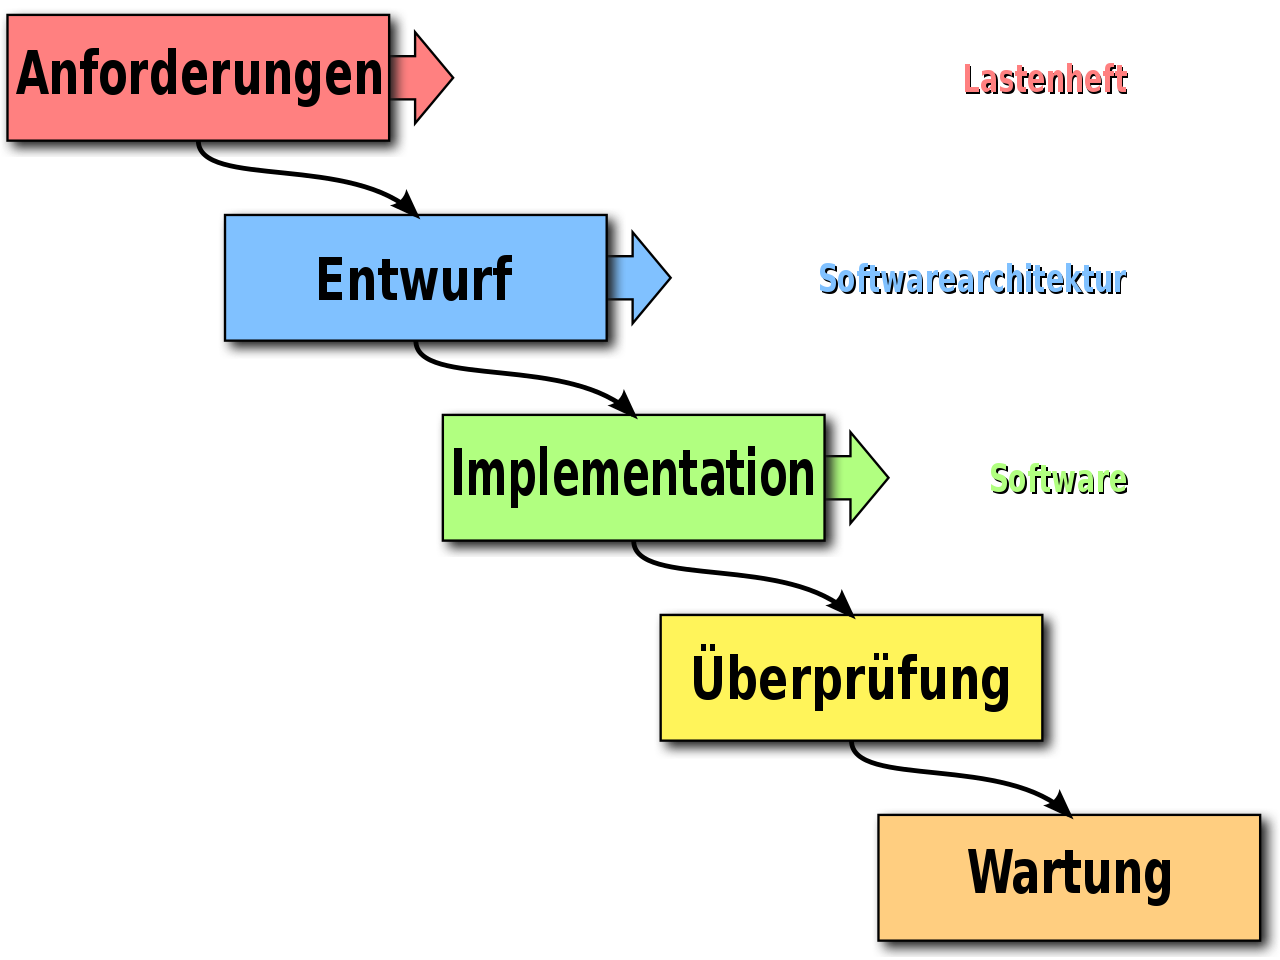
\includegraphics[width=0.7\textwidth]{res/Waterfall_model-de.svg.png} 
    \caption{Ablauf der Softwareentwicklung nach dem Wasserfallmodell} \cite{wasserfallmodellPic}
    \label{fig:wasserfallmodell}
\end{figure}

As you can see in the figure \ref{fig:wasserfallmodell}, the 
function grows near 0. Also, in the page \pageref{fig:wasserfallmodell} 
is the same example.

\myNewSection
\textbf{Stichpunkte:} 
Ermüdende Informationsberge sollten in einen Anhang verbannt werden. (Wichtige Begriffe definieren)
